%%%%%%%%%%%%%%%%%%%%%%%%%%%
% Este documento faz parte da classe cls-PFC-COEEL.cls
% NÃO ALTERE NENHUM DADO AQUI.
%%%%%%%%%%%%%%%%%%%%%%%%%%%
\pagestyle{EstiloPFC} % Estilo de página criado para o PFC do IFBA VDC
%%%% numeração da página em romano 
\pagenumbering{roman} 
%%%% espaçamento 1,5 entre linhas
\onehalfspacing
%%%%%%%%%%%%%%%%%%%%%%%%%%%%
%%%% CAPA 
%
% se é PFC faz capa de PFC

\ifpfc
    \CapaPFC
\fi 
    
% se é Relatório faz capa de Relatório
\ifrelatorio
    \CapaREL
\fi 

% se é Relatório faz capa de Pré-Projeto
\ifpreprojeto
    \CapaPREPROJETO
\fi 
%
%%%%%%%%%%%%%%%%%%%%%%%%%%%%
%%%% FOLHA DE ROSTO
% apenas para PFC
%
\ifpfc % se é PFC
    \newpage\clearpage\pagebreak
    \ifpdf\phantomsection\fi
    \addcontentsline{toc}{chapter}{Folha de Rosto}
    \FolhaRosto%
\fi 
\ifpreprojeto % se é Pré-Projeto
    \newpage\clearpage\pagebreak
    \ifpdf\phantomsection\fi
    \addcontentsline{toc}{chapter}{Folha de Rosto}
    \FolhaRosto%
\fi 
%
%%%%%%%%%%%%%%%%%%%%%%%%%%%%
%%%% FICHA CATALOGRÁFICA
% apenas para PFC
%
\ifpfc % se é PFC
    \newpage\clearpage\pagebreak
    \ifpdf\phantomsection\fi
    \addcontentsline{toc}{chapter}{Ficha Catalográfica}
    % inclua o PDF da ficha catalográfica feita pela biblioteca
    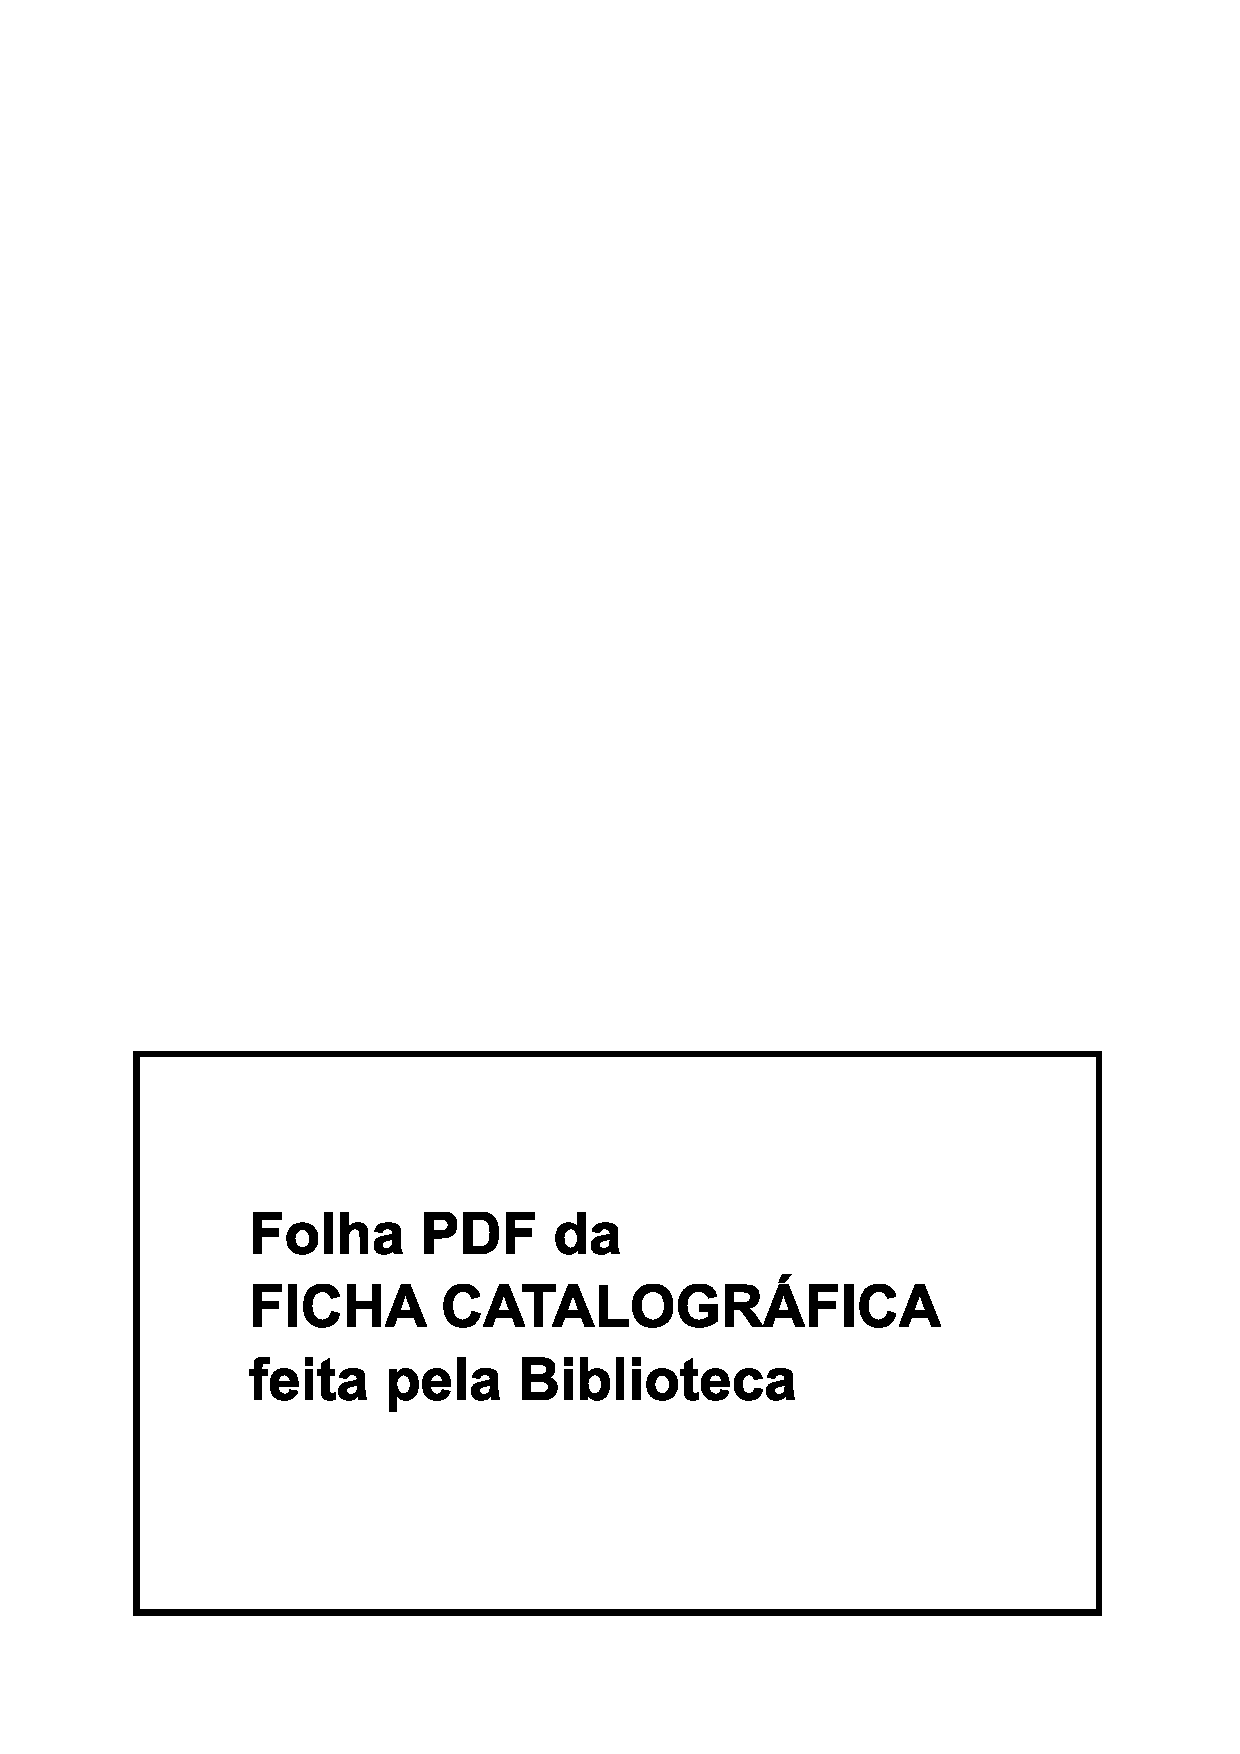
\includepdf[pages=1]{./PFC_Especificos/Ficha_Catalografica.pdf}
\fi 
%
%%%%%%%%%%%%%%%%%%%%%%%%%%%%
%%%% FOLHA DE APROVAÇÃO
% Apenas para PFC
%
\ifpfc % se é PFC
    \newpage\clearpage
    \ifpdf\phantomsection\fi
    \addcontentsline{toc}{chapter}{Folha de Aprovação}
    
    % inclua o PDF da folha de aprovação assinada digitalmente pelos membros da banca pelo SEI ou pelo SOU.GOV:

    % \includepdf[pages=1]{./PFC_Especificos/Folha_Aprovacao.pdf} % descomente esta linha quando for anexar o PDF

    % comente esta linha quando for anexar o PDF
    \include{./PFC_Especificos/b_FolhaAprovacao} 
\fi 
%
%%%%%%%%%%%%%%%%%%%%%%%%%%%
%%%% DEDICATÓRIA
% Apenas para PFC
%
\ifpfc % se é PFC
    \include{./PFC_Especificos/c_Dedicatoria}
\fi 
%
%%%%%%%%%%%%%%%%%%%%%%%%%%%%
%%%% AGRADECIMANTOS
% Apenas para PFC
%
\ifpfc % se é PFC
    \include{./PFC_Especificos/d_Agradecimentos}
\fi 
%
%%%%%%%%%%%%%%%%%%%%%%%%%%%%
%%%% RESUMO
% Apenas para PFC 
%
\ifpfc % se é PFC
    \newpage\clearpage
    \ifpdf\phantomsection\fi
    \addcontentsline{toc}{chapter}{Resumo}
    \include{./PFC_Especificos/e_Resumo}
\fi 
%
%%%%%%%%%%%%%%%%%%%%%%%%%%%%
%%%% ABSTRACT
% Apenas para PFC
%
\ifpfc % se é PFC
    \newpage\clearpage
    \ifpdf\phantomsection\fi
    \addcontentsline{toc}{chapter}{Abstract}
    \include{./PFC_Especificos/f_Abstract}
\fi 
%


%%%%%%%%%%%%%%%%%%%%%%%%%%%%
%%%% LISTA DE FIGURAS
% Apenas para PFC
%
\ifpfc % se é PFC
    \newpage\clearpage
    \ifpdf\phantomsection\fi
    \addcontentsline{toc}{chapter}{\listfigurename}
    \listoffigures
\fi 
%
%%%%%%%%%%%%%%%%%%%%%%%%%%%%
%%%% LISTA DE TABELAS
% Apenas para PFC
%
\ifpfc % se é PFC
    \clearpage\newpage
    \ifpdf\phantomsection\fi
    \addcontentsline{toc}{chapter}{\listtablename}
    \listoftables
\fi 
%
%%%%%%%%%%%%%%%%%%%%%%%%%%%%
%%%% LISTA DE CÓDIGOS
%
% Apenas para PFC
%
\ifpfc % se é PFC
    \clearpage\newpage
    \newcommand{\lstlistoflistingsname}{Lista de Códigos}
    \renewcommand{\lstlistingname}{Código}
    \addcontentsline{toc}{chapter}{Lista de Códigos\numberline{}}
    \lstlistoflistings
\fi 
%
%%%%%%%%%%%%%%%%%%%%%%%%%%%%
%%%% GLOSSÁRIO
%%%% LISTA DE SÍMBOLOS E SIGLAS
%
% https://pt.overleaf.com/learn/latex/Glossaries
%
% Glossário Apenas para PFC e Pré Projeto
%
\ifpfc % se é PFC
    \clearpage\newpage\pagebreak
    \renewcommand{\glossaryname}{Glossário: Símbolos e Siglas}
    \addcontentsline{toc}{chapter}{\glossaryname}
    \renewcommand{\pagelistname}{Páginas}%
    \printglossary[style=long3col-booktabs]
\fi
%
\ifpreprojeto % se é Pré Projeto de PFC
    \clearpage\newpage\pagebreak
    \renewcommand{\glossaryname}{Glossário: Símbolos e Siglas}
    \addcontentsline{toc}{chapter}{\glossaryname}
    \renewcommand{\pagelistname}{Páginas}%
    \printglossary[style=long3col-booktabs]
\fi
%
%%%%%%%%%%%%%%%%%%%%%%%%%%%%
%%%% SUMÁRIO
%
% Apenas para PFC e Pré-Projeto
%
\ifpfc % se é PFC
    \clearpage\pagebreak\newpage
    \renewcommand{\cftchapleader}{\cftdotfill{\cftdotsep}} % capítulos do sumário com linha de pontos
    \tableofcontents
\fi 
%
\ifpreprojeto  % se é Pré-Projeto
    \clearpage\pagebreak\newpage
    \renewcommand{\cftchapleader}{\cftdotfill{\cftdotsep}} % capítulos do sumário com linha de pontos
    \tableofcontents
\fi 
%
%%%%%%%%%%%%%%%%%%%%%%%%%%%%
%
\pagestyle{EstiloPFC} % estilo criado para este PFC
\clearpage\pagebreak\newpage
\onehalfspacing % espaçamento 1,5 entre linhas
\pagenumbering{arabic}  % numeração das páginas em algarismos arábicos
\makeatother %  restringir o uso do símbolo @ em comandos de macro
%
%%%%%%%%%%%%%%%%%%%%%%%%%%%%